\section{Положение металлов в Периодической системе. Общие физические и химические свойства металлов}

В периодической системе металлы расположены в начале периодов, (s- и некоторые p-элементы) а также в побочных подгруппах \ref{fig:2table}. В зависимости от конфигурации металлы делят на s-металлы (щелочные и щелочноземельные),  p-металлы, d-металлы и f-металлы (лантаноиды и актиноиды). Элементы группы проявляют схожие свойства.

\subsection{Общие свойства}

\begin{itemize}
    \item высокая тепло- и энергопроводность
    \item низкая электроотрицательность
    \item низкая энергия ионизации атомов
    \item восстановительные свойства простых веществ
    \item способность образовывать катионы $M^{n+}$, $n = 1-4$, но не проявляют отрицательные степени окисления
    \item твердое состояние при комнатной температуре(крроме ртути)
    \item в реакциях выступают в роли восстановителей:
    
    \ce{2Na^0 + Cl^0 -> 2Na^{+1}Cl^{-1}}
    
    \ce{2Al^0 + 3S^0 -> Al^{+3}_2S^{-2}_3}
    
    \item Восстановительная активность характеризуется электрохимическим рядом:
    
    \begin{figure}[H]
        \centering
        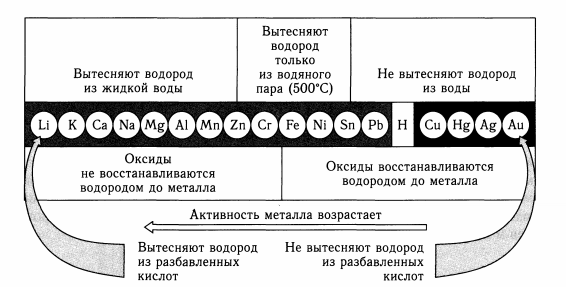
\includegraphics[width = \textwidth]{Pictures/12_metalrow.png}
        \caption{Электрохимический ряд напряжений}
        \label{fig:12row_metal}
    \end{figure}
    
    \item металлы до цинка способны вытеснять водород из воды, образуя гидроксиды:
    
    \ce{2K + 2H2O -> 2 KOH + H2}
    
    \item менее активные металлы могут реагировать с водяным паром, образуя оксид и водород
    
    \ce{3Fe+2H2O ->T[t] Fe3O4 + 2H2}
    
    \item металлы, стоящие левее водорода, вытесняют его из разбавленных кислот:
    
    \ce{Mg + 2HCl \text{(разб.)} -> MgCl2 + H2}
    
    \item более активные металлы могут вытеснять менее активные из солей, если обе соли(и исходная, и получившаяся) растворимы в воде:
    
    \ce{CuSO4 + Fe -> FeSO4 + Cu}
    
    
\end{itemize} 